% Measurement results / analysis / discussion:
% whatever you have done, you must comment it, compare it to other systems, evaluate it
% usually, adequate graphs help to show the benefits of your approach
% caution: each result/graph must be discussed! what’s the reason for this peak or why have you ovserved this effect

\chapter{Evaluation}\label{ch:evaluation}\glsresetall
To evaluate \project, we investigate its model prediction capabilities,






\section{Experimental Setup}\label{sec:experimental_setup}
We started by retrieving real-time data from $138$ different markets throughout $33$ days. The pairing coin of each market was Bitcoin. The interval between each data point was $5$ seconds, resulting in approximately $\numprint{570 000}$ samples per market. Over these days, we collected in total \SI{47}{\giga\byte} of data. The sources that we used to fetch data from was those we presented in the \autoref{ch:implementation}, namely Binance, CoinMarketCap, and aggregated data from multiple sources. 

\autoref{tab:feature_table} contains details regarding every feature that were fetched. The operation column describe how we decided to process a specific feature. The data were cleaned by removing features that we believe was unproductive in the detection of \ac{pd}, these were tagged as \emph{Removed}. The field that contains \emph{PoC}, was first interpolated and then calculated the percentage of change. We chose $10$ minutes for the time lag, because the time from where a \ac{pd} start to where it peak is around $10$ minutes, like described in \autoref{ch:background}. The field \emph{Imbalance} and \emph{Time} are the order book imbalance and how close the timestamp is on the hour.

\begin{table}
    \centering
    \begin{tabular}{|l|l|l|l|}
    \hline
            Source          & Symbol        & Feature Description           & Operation \\\hline
            Local           & $dt$          & Local timestamp               & Time      \\
            Binance         & $e$           & Event type                    & Removed   \\
            Binance         & $E$           & Event time                    & Removed   \\
            Binance         & $s$           & Symbol                        & Removed   \\
            Binance         & $P$           & Price change percent          & None      \\
            Binance         & $p$           & Price change                  & PoC       \\
            Binance         & $w$           & Weighted average price        & PoC       \\
            Binance         & $x$           & First trade(F)-1 price        & PoC       \\
            Binance         & $c$           & Last price                    & PoC       \\
            Binance         & $Q$           & Last quantity                 & PoC       \\
            Binance         & $b$           & Best bid price                & PoC       \\
            Binance         & $B$           & Best bid quantity             & PoC       \\
            Binance         & $a$           & Best ask price                & PoC       \\
            Binance         & $A$           & Best ask quantity             & PoC       \\
            Binance         & $o$           & Open price                    & PoC       \\
            Binance         & $h$           & High Price                    & PoC       \\
            Binance         & $l$           & Low Price                     & PoC       \\
            Binance         & $v$           & Base asset volume             & PoC       \\
            Binance         & $q$           & Quote asset volume            & PoC       \\
            Binance         & $O$           & Statistics open time          & Removed   \\
            Binance         & $C$           & Statistics close time         & Removed   \\
            Binance         & $F$           & First trade ID                & Removed   \\
            Binance         & $L$           & Last trade ID                 & Removed   \\
            Binance         & $n$           & Total number of trades        & PoC       \\
            Binance         & $ap\_[0-4]$   & $5$x depth - asks price       & PoC       \\
            Binance         & $av\_[0-4]$   & $5$x depth - asks volume      & PoC       \\
            Binance         & $bp\_[0-4]$   & $5$x depth - bids price       & PoC       \\
            Binance         & $av\_[0-4]$   & $5$x depth - asks volume      & PoC       \\
            Binance         & $dep$         & Depth imbalance               & Imbalance \\
            ccxt            & $oc$          & Aggregated open price         & PoC       \\
            ccxt            & $hc$          & Aggregated high price         & PoC       \\
            ccxt            & $lc$          & Aggregated low price          & PoC       \\
            ccxt            & $cc$          & Aggregated close price        & PoC       \\
            ccxt            & $ic$          & Exchange to market rate       & None      \\
            CoinMarketCap   & $cap$         & Capitalization rate           & None      \\
    \hline
    \end{tabular}
    \caption[Features used]{This is all the features we fetched and used to train our model.}
    \label{tab:feature_table}
\end{table}


We used the anomaly detection algorithm which we have previously described in \autoref{ch:design} to pinpoint \ac{pd} intervals. We fetched \ac{ohlc} values that span over the period we collected data, and these \ac{ohlc} values had an interval of $1$ hour. The threshold parameters we chose for the algorithm is a price increase of $1.10$ and a volume of increase threshold of $3.00$, and the time lag we chose was $6$ hour. By using this algorithm we were able to identify in total $280$ anomalies. Of these anomalies we manually removed $80$, which we believe was false.

\autoref{fig:label_true} shows three \acp{pd} charts we believe was true, while \autoref{fig:label_false} shows three \ac{pd} charts we believe was false. From \autoref{fig:label_true} the price suddenly increases by approximately $20\%$. This sudden increase only lasts for a few minutes before the price dumps straight down to what it was before the increase. These price characteristics are exactly like the patterns we have previously defined that describe \acp{pd}. 

%From the other figures that illustrate anomalies that we believe do not contain \acp{pd} (\autoref{fig:label_false}). 
\autoref{fig:label_false} on the other hand show anomalies that we do not believe is \acp{pd}. It seems like the price fluctuates substantially, and the price does indeed fluctuate, but the scale in these charts is different from the other. The difference between the lowest and the highest price is only around $5\%$ in each of the anomalies. If any these allegedly false \acp{pd} is true, then these fail in raising the price significantly. In addition to having a longer time scale to those we believe is true as there are no sudden increase in price, which breaks the current patterns of \acp{pd}.

\if0
\begin{figure}
    \centering
    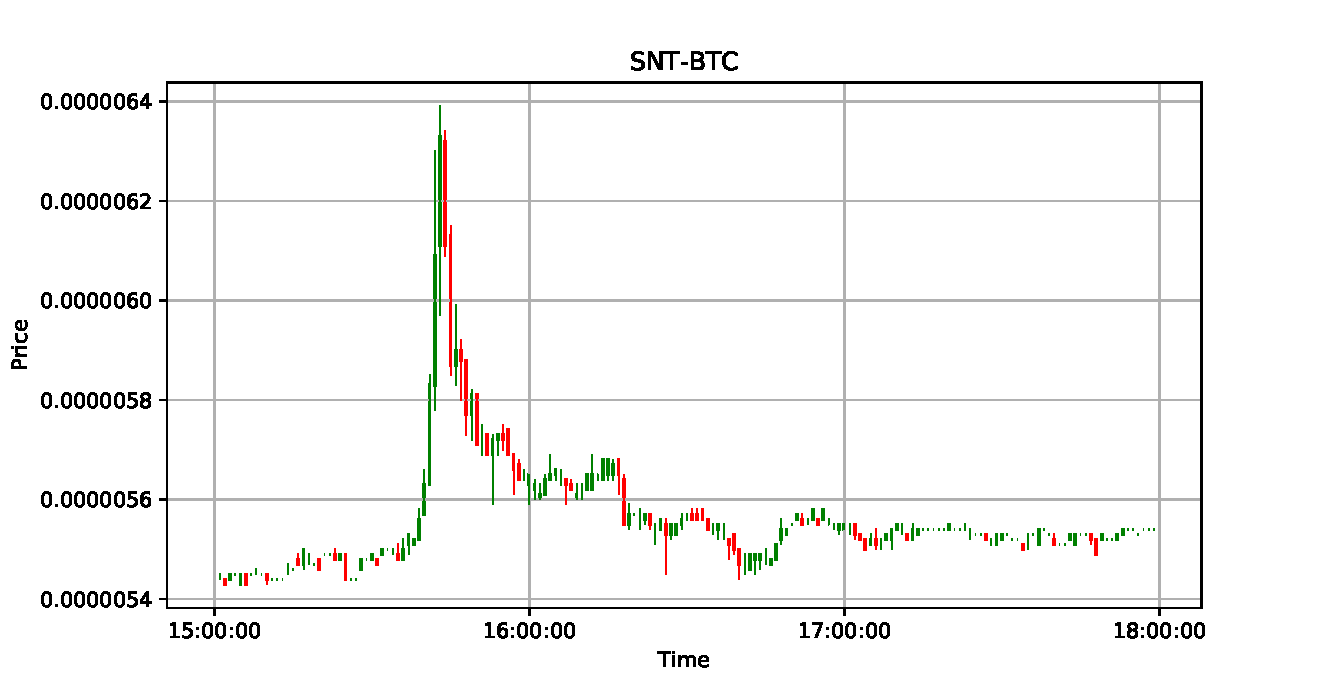
\includegraphics[width=\textwidth]{true_1.pdf}
    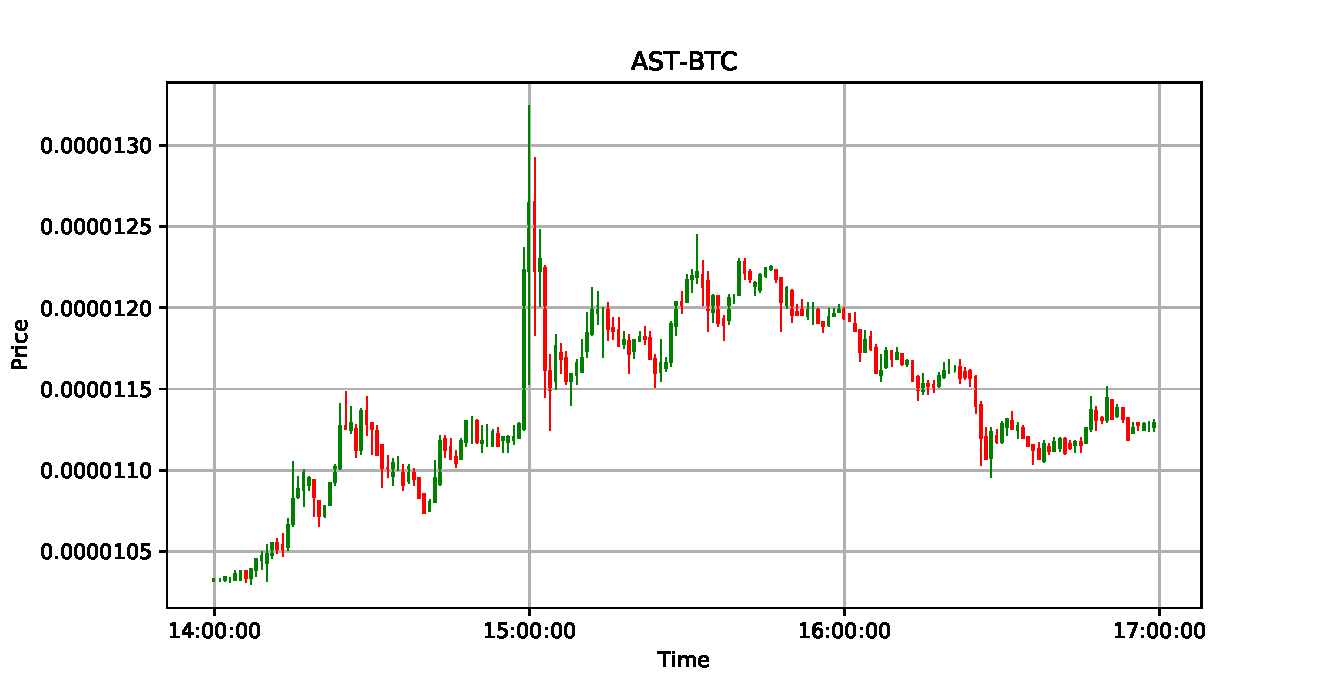
\includegraphics[width=\textwidth]{true_2.pdf}
    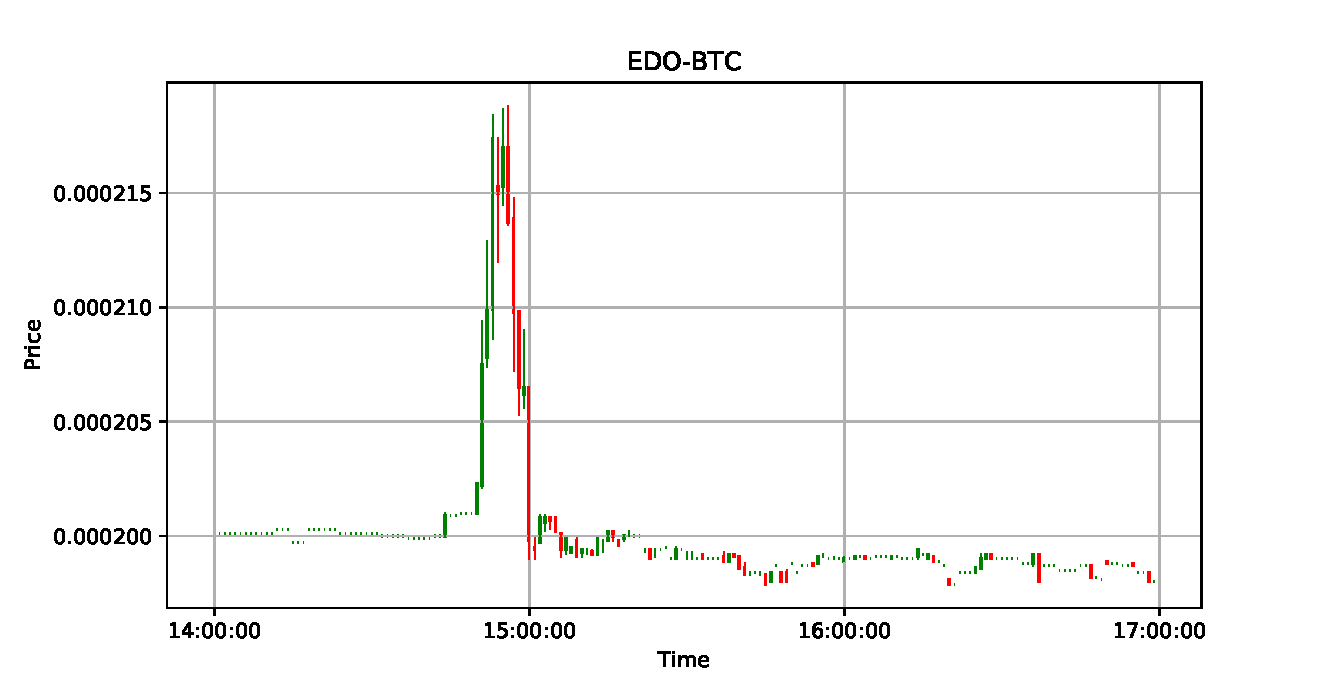
\includegraphics[width=\textwidth]{true_3.pdf}
    \caption{Anomalies that seems like a \ac{pd}}
    \label{fig:label_true}
\end{figure}

\begin{figure}
    \centering
    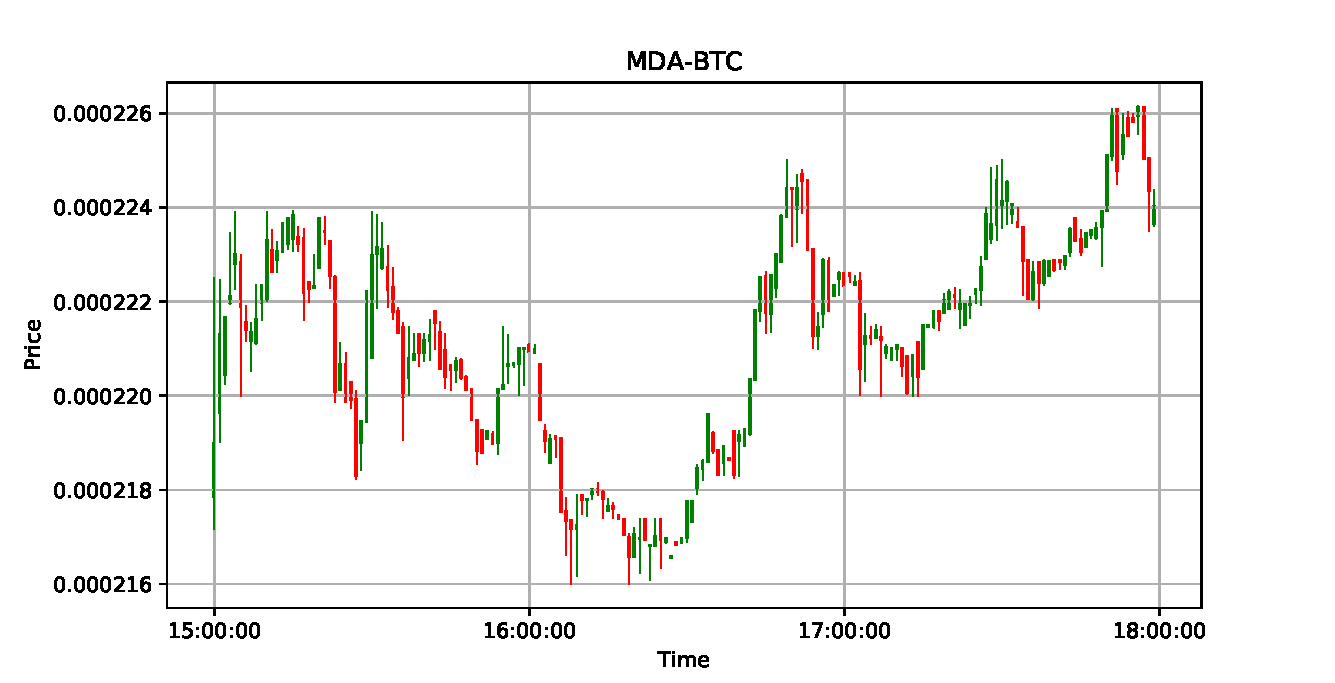
\includegraphics[width=\textwidth]{false_1.pdf}
    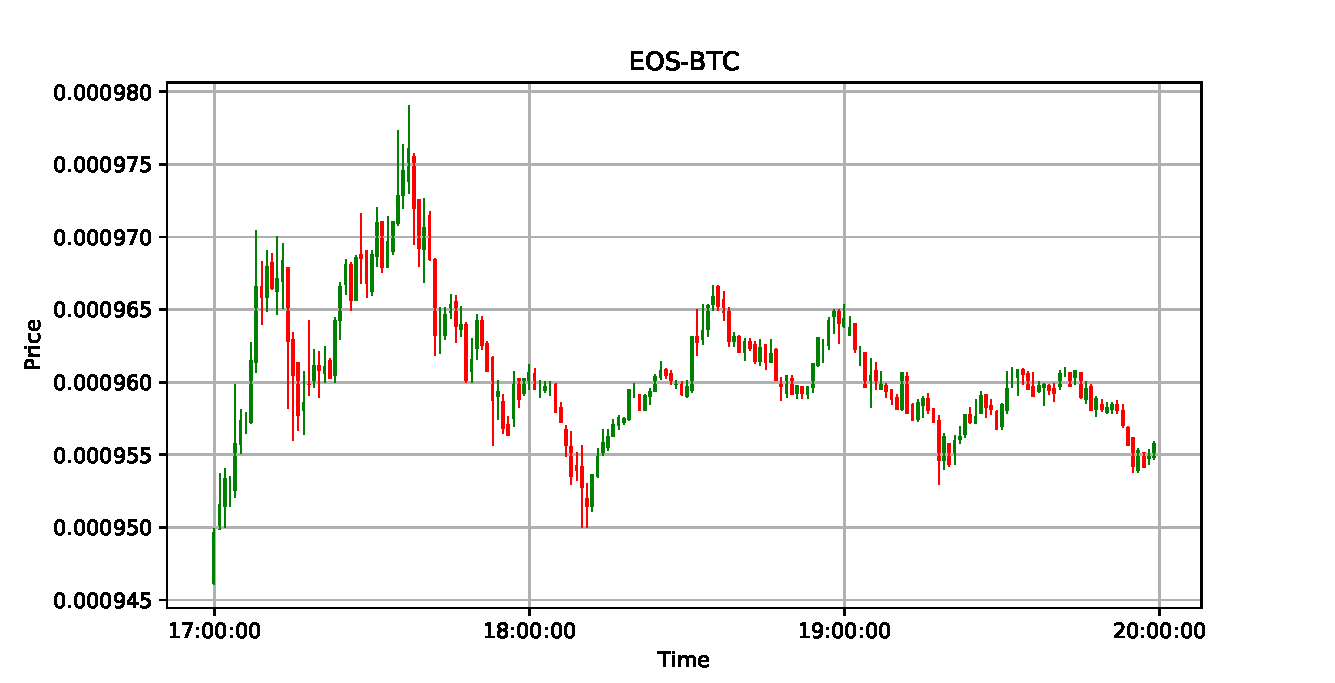
\includegraphics[width=\textwidth]{false_2.pdf}
    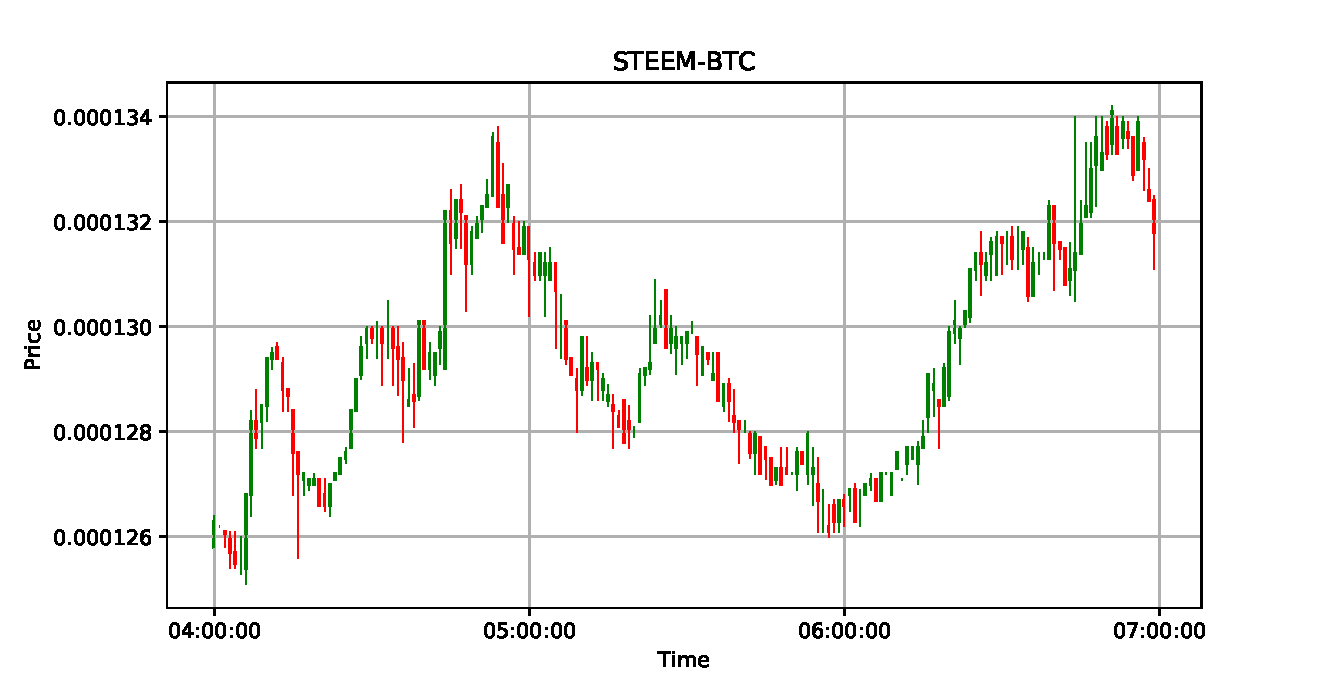
\includegraphics[width=\textwidth]{false_3.pdf}
    \caption{Anomalies that not seems like a \ac{pd}.}
    \label{fig:label_false}
\end{figure}
\fi

\begin{figure}[hbt!]
    \centering
    \begin{subfigure}{.49\textwidth}
        \centering
        \begin{subfigure}{\textwidth}
            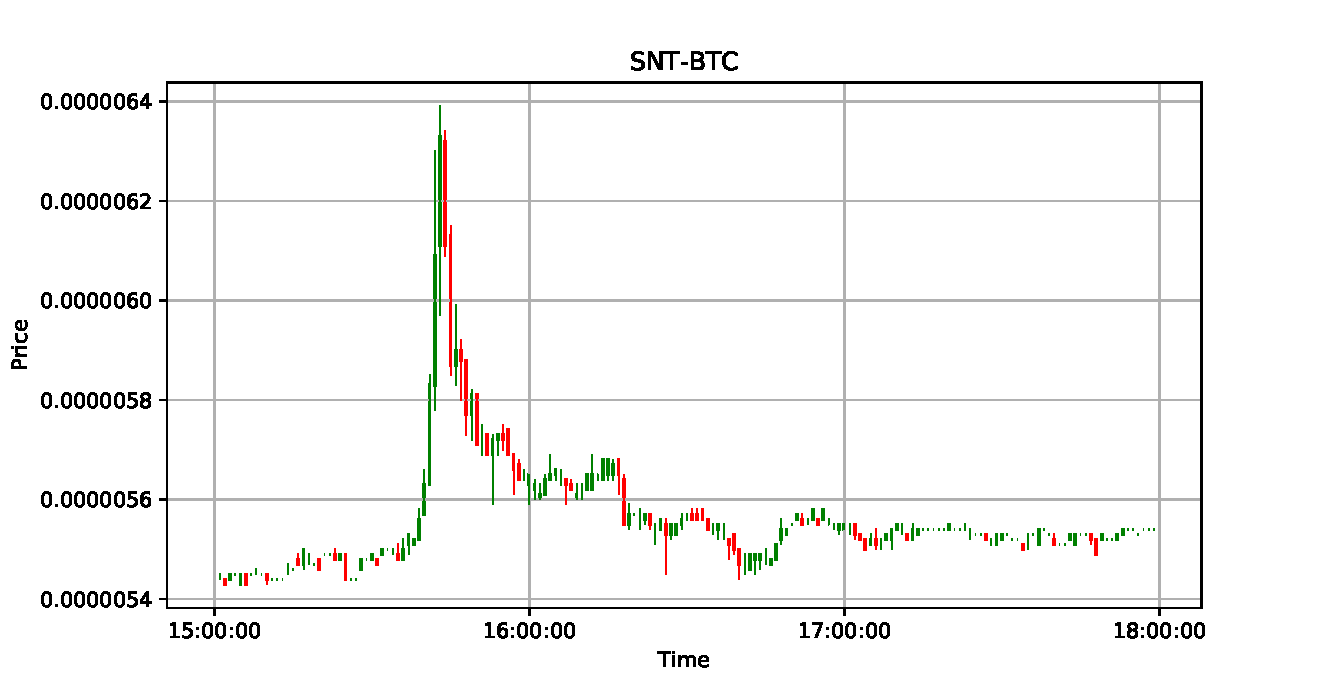
\includegraphics[trim={3.6cm 1.3cm 2.95cm 1.3cm},clip,width=\textwidth]{true_1.pdf}
            \caption*{SNT-BTC}
        \end{subfigure}
        \begin{subfigure}{\textwidth}
            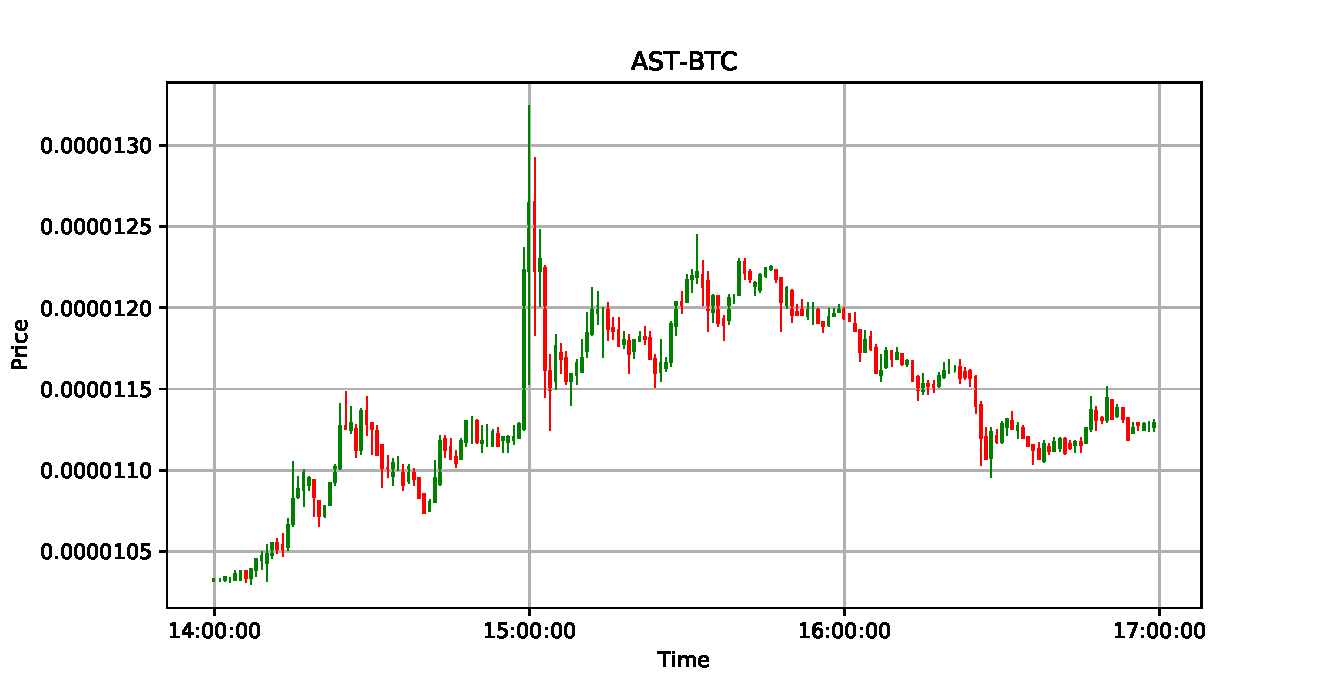
\includegraphics[trim={3.6cm 1.3cm 2.95cm 1.3cm},clip,width=\textwidth]{true_2.pdf}
            \caption*{AST-BTC}
        \end{subfigure}
        \begin{subfigure}{\textwidth}
            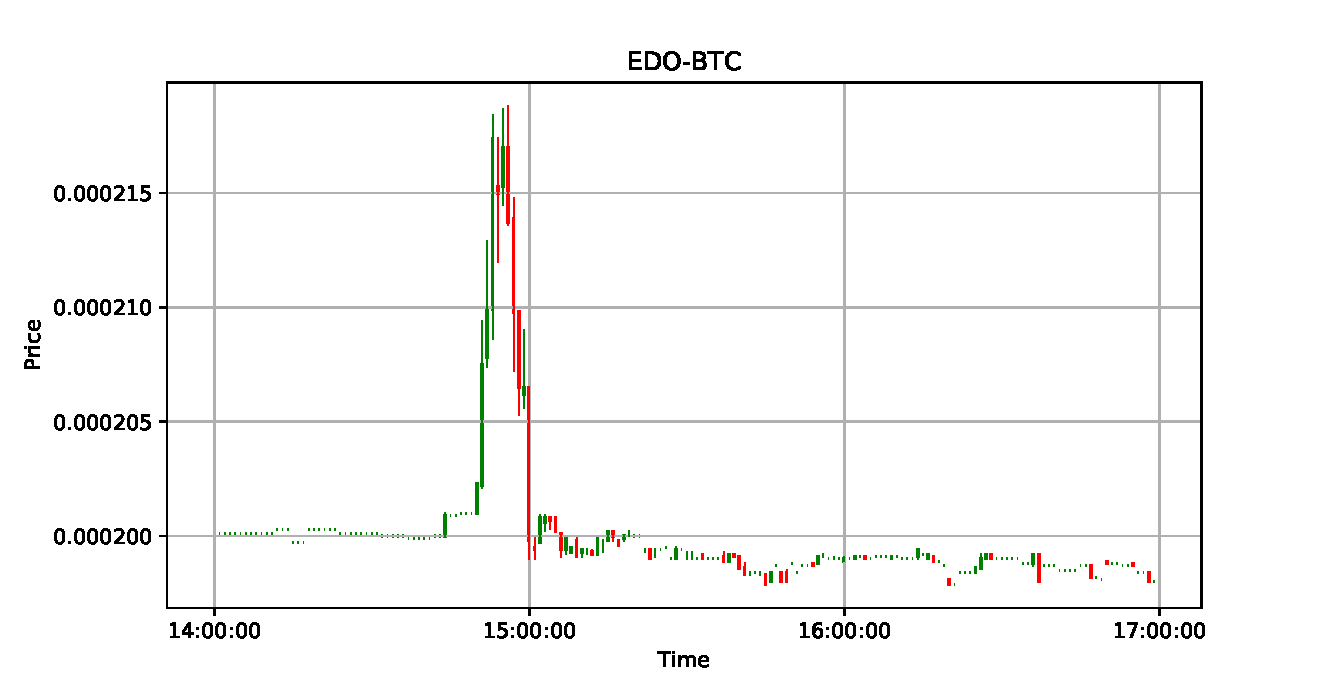
\includegraphics[trim={3.6cm 1.3cm 2.95cm 1.3cm},clip,width=\textwidth]{true_3.pdf}
            \caption*{EDO-BTC}
        \end{subfigure}
        \caption{Anomalies that seems like a \ac{pd}.}
        \label{fig:label_true}
    \end{subfigure}
    \hfill
    \begin{subfigure}{.49\textwidth}
        \centering
        \begin{subfigure}{\textwidth}
            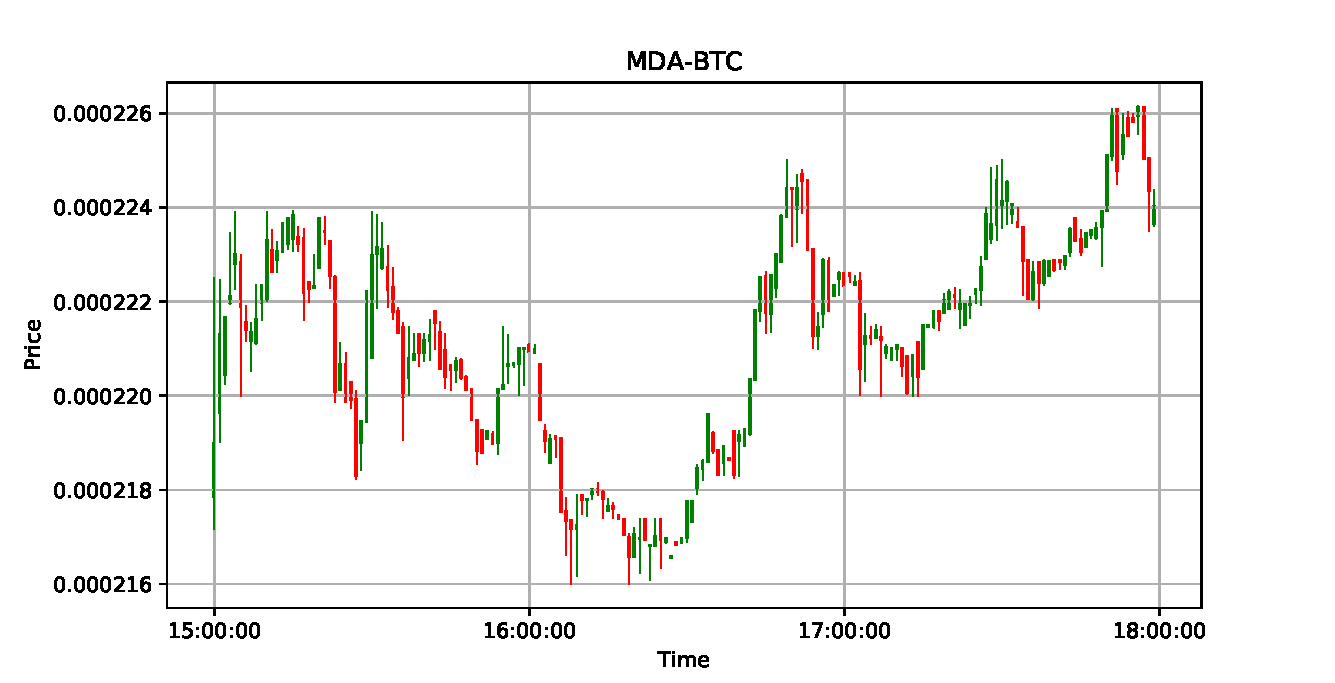
\includegraphics[trim={3.6cm 1.3cm 2.95cm 1.3cm},clip,width=\textwidth]{false_1.pdf}
            \caption*{MDA-BTC}
        \end{subfigure}
        \begin{subfigure}{\textwidth}
            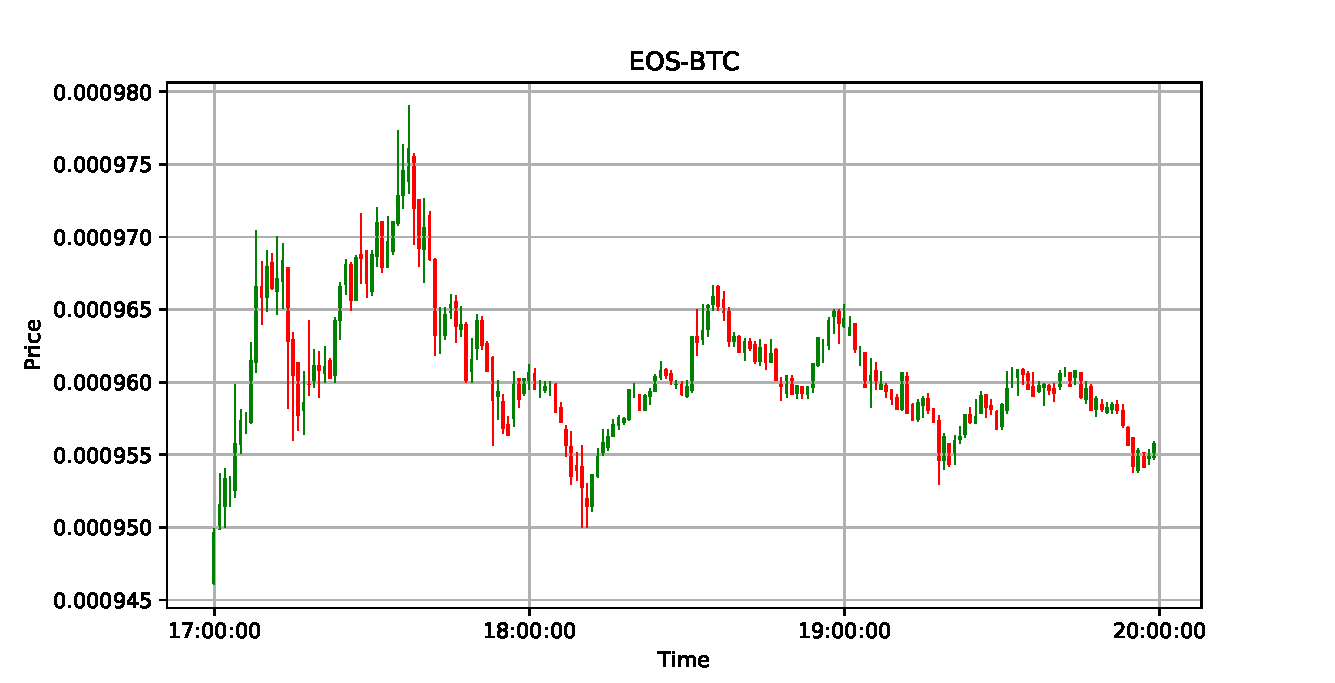
\includegraphics[trim={3.6cm 1.3cm 2.95cm 1.3cm},clip,width=\textwidth]{false_2.pdf}
            \caption*{EOS-BTC}
        \end{subfigure}
        \begin{subfigure}{\textwidth}
            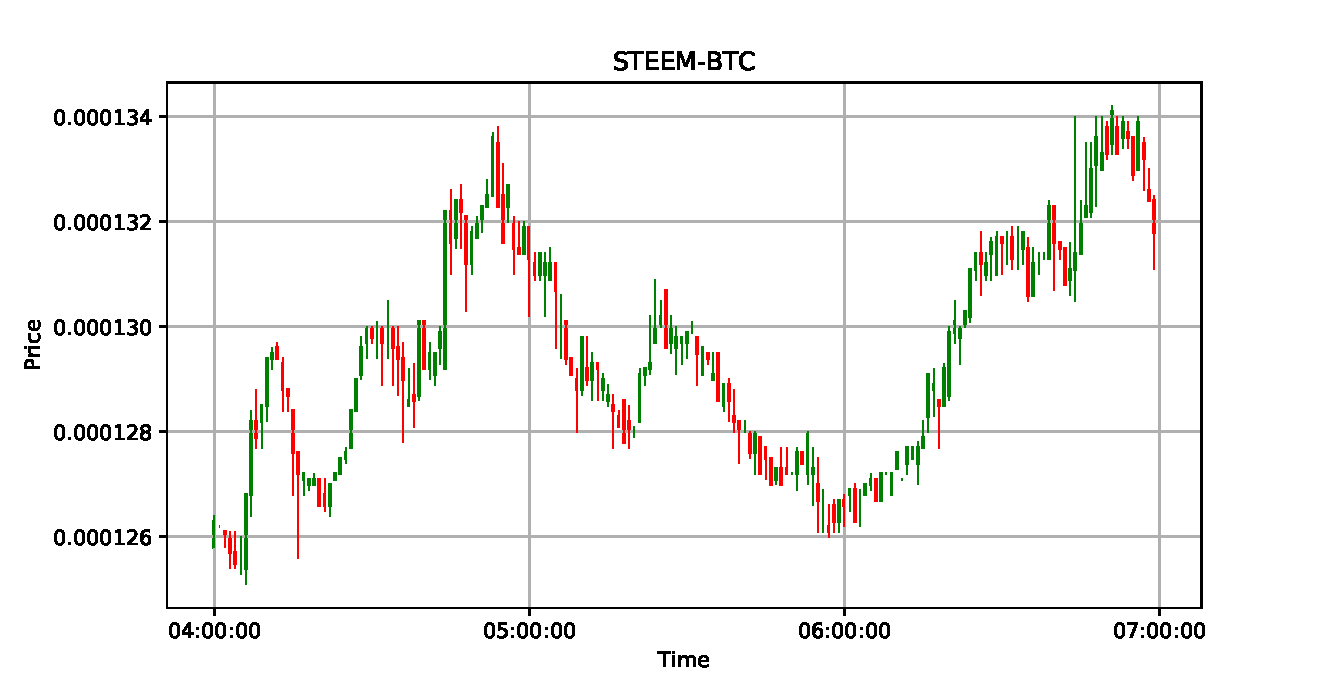
\includegraphics[trim={3.6cm 1.3cm 2.95cm 1.3cm},clip,width=\textwidth]{false_3.pdf}
            \caption*{STEEM-BTC}
        \end{subfigure}
        \caption{Anomalies that not seems like a \ac{pd}.}
        \label{fig:label_false}    
    \end{subfigure}
    \caption[Anomalies in the dataset]{These anomalies are only $6$ out of $280$ anomalies that were collected. The three anomalies on right were later removed as we believe those are false, while the three on the left we kept as they seems legitimate.}
\end{figure}


To create a dataset, we used the anomalies to label all the processed, collected data. The generated dataset was then normalized by using the min-max normalization method. We split the dataset into a training set and a test set. The training set was consist of $75\%$ of the dataset, resulting in data from approximately $104$ markets, while the test set contains the remaining $25\%$ of the markets, resulting in $33$ markets. The training dataset was undersampled in order to create a balanced dataset.

The network we used was a \ac{lstm} network, where its hidden layer contains a single layer with $50$ \ac{lstm} cells, where each cell had a "short memory" of $10$ points, which results in $50$ seconds of memory considering that interval between each sample is $5$ seconds. We also added dropout to prevent over-fitting as \ac{lstm} cells tend to overfit their training data often~\cite{overfit}. The output layer contained a single perceptron. The optimizer we used was \emph{adam}, which is an extension to stochastic gradient descent~\cite{kingma2014adam}, the optimizer has shown that the model's weights will converge faster that results in greater performance rapidly~\cite{adam}. The network was trained in over $5000$ epochs with the training dataset, where the batch size was $10$. To define the performance of the network, we classified all the samples in the test dataset and rounded the probabilistic prediction to either $0$ (\ac{pd}) or $1$ (not \ac{pd}). 

The computer we used to train our model with had the following specifications:
\begin{itemize}
    \item CPU - Intel Xeon E5-1620 \SI{3.9}{\giga\hertz}
    \item RAM - \SI{64}{\gibi\byte} DDR3 
    \item GPU - Nvidia GeForce GTX 770
\end{itemize}
%\newpage

\section{Results}
The first metric we use is a confusion matrix, which is structured like \autoref{tab:confmat}. A confusion matrix shows the number of correct and incorrect classified samples, and help define further scores. True positive $tp$ are samples that are correctly classified as \ac{pd}, while true negative, $tn$, is samples that are correctly classified as not \ac{pd}. $fp$ are samples that are incorrect classified as \ac{pd}, and false negatives, $fn$, are samples that are \ac{pd}, but classified as not \ac{pd}. $p$ and $n$ are the true total numbers of samples in each class, while $p'$ and $n'$ are the total numbers of predicted samples in each class. Finally, $N$ is the total number of samples.

\begin{table}
    \centering
    \begin{tabular}{|c|c|c|c|}\hline
                &   \multicolumn{3}{c|}{Predicted class}\\\hline
    True class  &  Positive             & Negative              & Total \\\hline
    Positive    & $tp$: true positive   & $fn$: false negative  & $p$   \\
    Negative    & $fp$: false positive  & $tn$: true negative   & $n$   \\\hline
    Total       & $p'$                  & $n'$                  & $N$   \\\hline
    \end{tabular}
    \caption{Confusion matrix}
    \label{tab:confmat}
\end{table}
\begin{table}
        \centering
        \begin{tabularx}{\textwidth}{ |R|R|R|R| }\hline
                    &   \multicolumn{3}{c|}{Predicted class}\\\hline
        True class  & Positive              & Negative              & Total                 \\\hline
        Positive    & $\numprint{7910}$     & $\numprint{911}$      & $\numprint{8821}$     \\
        Negative    & $\numprint{388795}$   & $\numprint{17933021}$ & $\numprint{18321816}$ \\\hline
        Total       & $\numprint{396705}$   & $\numprint{17933932}$ & $\numprint{18330637}$ \\\hline
        \end{tabularx}
        \caption{\project's confusion matrix}
        \label{tab:model_performance}
\end{table}

As we can see from \autoref{tab:model_performance}, the test dataset, as well as the training dataset, is hugely imbalanced. Only $\numprint{8821}$ samples are \ac{pd}, while $\numprint{18321816}$ is not a \ac{pd}. Over one of every $\numprint{2000}$ sample is a \ac{pd}! \autoref{tab:model_performance} contains the aggregated results of every market we tested the model on. The confusion matrix of each market will be presented later. It is more feasible to present the model's prediction capabilities by using a single matrix, instead of going through all the market's confusion matrices.

\begin{table}
    \centering
    \begin{tabular}{|c|c|r|}\hline
    Name        & Formula       &   Result      \\\hline
    error       & $(fp+fn)/N$   &   $0.0217$    \\
    accuracy    & $(tp+tn)/N$   &   $0.9782$    \\\hline
    tp-rate     & $tp/p$        &   $0.8967$    \\
    fp-rate     & $fp/n$        &   $0.0212$    \\\hline
    sensitivity & $tp/p$        &   $0.8967$    \\
    specificity & $tn/n$        &   $0.9787$    \\\hline
    recall      & $tp/p$        &   $0.8967$    \\
    precision   & $tp/p'$       &   $0.0199$    \\\hline
    \end{tabular}
    \caption{Performance measure}
    \label{tab:performance}
\end{table}

From \autoref{tab:performance}, we see various metrics that we can use when defining the capabilities of the \ac{lstm} network, the metrics \emph{accuracy} and \emph{error}, are measures that are opposite of each other. The accuracy is the percentage of how many samples we classified correct. The error, is the percentage how many samples we misclassified.

\begin{figure}[ht]
    \centering
    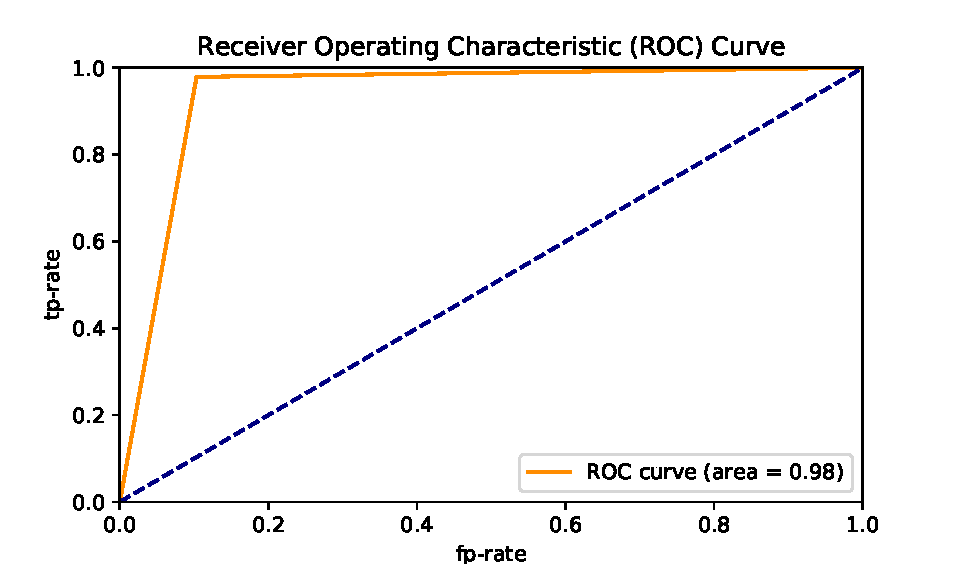
\includegraphics[width=\textwidth]{results/roc.pdf}
    \caption[\project's \acf{roc} curve]{Roc Curve}
    \label{fig:roc}
\end{figure} 

The tp-rate is percentage of how often we correctly classify \ac{pd} samples. So given a \ac{pd} sample, there an $89.67\%$ chance of classifying it correctly. The fp-rate is similar in terms of, given a negative sample. Then there is a $2.12\%$ change of classifying it at as a \acp{pd}. These measures can also be visualized through \ac{roc} curve illustrated in \autoref{fig:roc}. It gives us a visual perspective of the performance of the model. Ideally, a classifier has a tp-rate of $1$ and an fp-rate of $0$, and a classifier is better the more its \ac{roc} curve gets closer to the upper-left corner. On the diagonal, we make as many true decisions as false ones, and this is the worst case~\cite[p.~563]{alpaydin2014introduction}. Our \ac{roc} curve also shows that our model has accurate predictable capabilities. The \ac{auc} score represents the probability that a randomly chosen positive example is correctly classified ranked with greater suspicion than a randomly chosen negative example~\cite{bradley1997use}.
The \emph{sensitivity} and \emph{specificity} balance the classes, they tells us, given a negative or positive samples, what is the percentage of classifying it correctly. The sensitivity, is the percentage of given a positive sample, the percentage of classifying it correctly, is $89.67\%$. The specificity, is the opposite, given a negative sample, the percentage of classifying it correctly is $97.87\%$. 

Clearly, the metrics we presented now shows that the model has good predictable capabilities. However, the metrics that reveal the flaws of the model, are the measures \emph{recall} and \emph{precision}. Recall are exactly like the tp-rate and sensitivity, it is the percentage of, given a \ac{pd} sample, then there is $89.67\%$ chance of classifying it correctly. \emph{precision} on the other hand, is, if classifying a sample as a \ac{pd}, then, what is the percentage that the sample truly is a \ac{pd}. In our case, a disappointing $1.99\%$. so whenever our model predicts a \ac{pd}, then there is only a $1.99\%$ that it is correct, and this results in plenty of false alarms.

\begin{align}\label{eq:f_score}
    F_\beta &= (1+\beta^2) \cdot \frac{\text{precision} \cdot \text{recall}}{(\beta^2\cdot\text{precision}) + \text{recall}},\quad
    \begin{cases} 
    F_{0.5} &= 0.0247\\ 
    F_1     &= 0.0389\\ 
    F_2     &= 0.0912\\ 
    \end{cases}
\end{align}

A frequently used score that relies on recall and precision is the \emph{f-score}. The f-score formula is showed in \autoref{fig:f_score}, and an ideal f-score is $1$, and the worst is $0$. This measure is flexible in terms that we can weigh both recall and precision differently by adjusting the parameter $\gamma$. Where the closer $\gamma$ is to $0$, the more we weigh precision, when $\gamma$ is $1$ we wight them equally, and finally when $\gamma$ is over $1$, we weigh recall most. As we see, when weighing precision most, by giving  $\gamma=0.5$, the score only yield $0.0247$. When equally weighing them, by giving $\gamma=1$, the score increase slightly. Finally, when weighting recall most, the score is $0.0912$, which is better than the other.

\autoref{tab:results} shows the confusion matrix of each classified market. We colorize the cells to visualize the performance of the model. The green cells on the diagonal contain the number of correctly classified sample, and the color illustrates the percentage of correctly classified samples in its class — the more intense green on the diagonal, the more correct predictions the model does. The red cell on the anti-diagonal consist of the number of misclassified samples, and this color represents the percentage of misclassified samples in its class. The red present the same as green, only that the insensitivity presents misclassification. How white cells are has a split meaning, it is a good sign on the anti-diagonal (red), but an awful one on the diagonal (green). A noticeable observation, there are markets containing no \acp{pd}. They are colored green in the true positive cell and e white in the false positive cell.

\begin{table}[H]
        \centering
        \begin{tabularx}{\textwidth}{ |R|R||R|R||R|R| }
                \multicolumn{2}{c}{WABI-BTC} & \multicolumn{2}{c}{MITH-BTC} & \multicolumn{2}{c}{ETH-BTC} \\\hline
                $\numprint{376}$\cellcolor{green!91} & $\numprint{36}$\cellcolor{red!9} & $\numprint{0}$\cellcolor{green!0} & $\numprint{2}$\cellcolor{red!100} & $\numprint{0}$\cellcolor{green!100} & $\numprint{0}$\cellcolor{red!0} \\
                $\numprint{23440}$\cellcolor{red!5} & $\numprint{531622}$\cellcolor{green!95} & $\numprint{26798}$\cellcolor{red!5} & $\numprint{528675}$\cellcolor{green!95} & $\numprint{0}$\cellcolor{red!0} & $\numprint{555474}$\cellcolor{green!100} \\
                \hline
                \addlinespace[.2cm]

                \multicolumn{2}{c}{XRP-BTC} & \multicolumn{2}{c}{BTT-BTC} & \multicolumn{2}{c}{OST-BTC} \\\hline               
                $\numprint{0}$\cellcolor{green!100} & $\numprint{0}$\cellcolor{red!0} & $\numprint{0}$\cellcolor{green!100} & $\numprint{0}$\cellcolor{red!0} & $\numprint{488}$\cellcolor{green!90} & $\numprint{53}$\cellcolor{red!10} \\
                $\numprint{0}$\cellcolor{red!0} & $\numprint{555474}$\cellcolor{green!100} & $\numprint{3400}$\cellcolor{red!1} & $\numprint{552074}$\cellcolor{green!99} & $\numprint{8705}$\cellcolor{red!2} & $\numprint{546228}$\cellcolor{green!98} \\
                \hline
                \addlinespace[.2cm]

                \multicolumn{2}{c}{CDT-BTC} & \multicolumn{2}{c}{GNT-BTC} & \multicolumn{2}{c}{TRX-BTC} \\\hline               
                $\numprint{407}$\cellcolor{green!88} & $\numprint{51}$\cellcolor{red!12} & $\numprint{375}$\cellcolor{green!78} & $\numprint{105}$\cellcolor{red!22} & $\numprint{0}$\cellcolor{green!100} & $\numprint{0}$\cellcolor{red!0} \\
                $\numprint{18303}$\cellcolor{red!4} & $\numprint{536713}$\cellcolor{green!96} & $\numprint{20994}$\cellcolor{red!4} & $\numprint{534000}$\cellcolor{green!96} & $\numprint{289}$\cellcolor{red!1} & $\numprint{555185}$\cellcolor{green!99} \\
                \hline
                \addlinespace[.2cm]

                \multicolumn{2}{c}{MTH-BTC} & \multicolumn{2}{c}{DLT-BTC} & \multicolumn{2}{c}{SC-BTC} \\\hline                
                $\numprint{487}$\cellcolor{green!97} & $\numprint{16}$\cellcolor{red!3} & $\numprint{584}$\cellcolor{green!87} & $\numprint{85}$\cellcolor{red!13} & $\numprint{0}$\cellcolor{green!100} & $\numprint{0}$\cellcolor{red!0} \\
                $\numprint{12032}$\cellcolor{red!3} & $\numprint{542939}$\cellcolor{green!97} & $\numprint{19223}$\cellcolor{red!3} & $\numprint{535580}$\cellcolor{green!97} & $\numprint{7234}$\cellcolor{red!2} & $\numprint{548240}$\cellcolor{green!98} \\
                \hline
                \addlinespace[.2cm]

                \multicolumn{2}{c}{SNT-BTC} & \multicolumn{2}{c}{XEM-BTC} & \multicolumn{2}{c}{VIB-BTC} \\\hline                
                $\numprint{323}$\cellcolor{green!88} & $\numprint{40}$\cellcolor{red!12} & $\numprint{0}$\cellcolor{green!100} & $\numprint{0}$\cellcolor{red!0} & $\numprint{674}$\cellcolor{green!99} & $\numprint{7}$\cellcolor{red!1} \\
                $\numprint{8138}$\cellcolor{red!2} & $\numprint{546973}$\cellcolor{green!99} & $\numprint{914}$\cellcolor{red!1} & $\numprint{554559}$\cellcolor{green!99} & $\numprint{22358}$\cellcolor{red!5} & $\numprint{532435}$\cellcolor{green!95} \\
                \hline
                \addlinespace[.2cm]

                \multicolumn{2}{c}{MTL-BTC} & \multicolumn{2}{c}{HC-BTC} & \multicolumn{2}{c}{STORM-BTC} \\\hline             
                $\numprint{477}$\cellcolor{green!93} & $\numprint{36}$\cellcolor{red!7} & $\numprint{251}$\cellcolor{green!57} & $\numprint{188}$\cellcolor{red!43} & $\numprint{0}$\cellcolor{green!100} & $\numprint{0}$\cellcolor{red!0} \\
                $\numprint{29687}$\cellcolor{red!6} & $\numprint{525274}$\cellcolor{green!94} & $\numprint{5213}$\cellcolor{red!1} & $\numprint{549822}$\cellcolor{green!99} & $\numprint{14995}$\cellcolor{red!3} & $\numprint{540479}$\cellcolor{green!97} \\
                \hline
                \addlinespace[.2cm]

                \multicolumn{2}{c}{INS-BTC} & \multicolumn{2}{c}{LUN-BTC} & \multicolumn{2}{c}{NXS-BTC} \\\hline               
                $\numprint{0}$\cellcolor{green!0} & $\numprint{1}$\cellcolor{red!100} & $\numprint{792}$\cellcolor{green!93} & $\numprint{57}$\cellcolor{red!7} & $\numprint{0}$\cellcolor{green!100} & $\numprint{0}$\cellcolor{red!0} \\
                $\numprint{7032}$\cellcolor{red!2} & $\numprint{548439}$\cellcolor{green!98} & $\numprint{12443}$\cellcolor{red!3} & $\numprint{542182}$\cellcolor{green!97} & $\numprint{6554}$\cellcolor{red!1} & $\numprint{548920}$\cellcolor{green!99} \\
                \hline
                \addlinespace[.2cm]

                \multicolumn{2}{c}{TNB-BTC} & \multicolumn{2}{c}{NPXS-BTC} & \multicolumn{2}{c}{ZRX-BTC} \\\hline               
                $\numprint{441}$\cellcolor{green!99} & $\numprint{3}$\cellcolor{red!1} & $\numprint{0}$\cellcolor{green!100} & $\numprint{0}$\cellcolor{red!0} & $\numprint{0}$\cellcolor{green!100} & $\numprint{0}$\cellcolor{red!0} \\
                $\numprint{47144}$\cellcolor{red!9} & $\numprint{507886}$\cellcolor{green!91} & $\numprint{3381}$\cellcolor{red!1} & $\numprint{552093}$\cellcolor{green!99} & $\numprint{10138}$\cellcolor{red!2} & $\numprint{545336}$\cellcolor{green!98} \\
                \hline
                \addlinespace[.2cm]

                \multicolumn{2}{c}{VET-BTC} & \multicolumn{2}{c}{RCN-BTC} & \multicolumn{2}{c}{ETC-BTC} \\\hline                
                $\numprint{0}$\cellcolor{green!100} & $\numprint{0}$\cellcolor{red!0} & $\numprint{487}$\cellcolor{green!95} & $\numprint{26}$\cellcolor{red!5} & $\numprint{160}$\cellcolor{green!84} & $\numprint{30}$\cellcolor{red!16} \\
                $\numprint{1321}$\cellcolor{red!2} & $\numprint{554153}$\cellcolor{green!98} & $\numprint{10697}$\cellcolor{red!2} & $\numprint{544264}$\cellcolor{green!98} & $\numprint{2890}$\cellcolor{red!1} & $\numprint{552394}$\cellcolor{green!99} \\
                \hline
                \addlinespace[.2cm]

                \multicolumn{2}{c}{SNM-BTC} & \multicolumn{2}{c}{SKY-BTC} & \multicolumn{2}{c}{LOOM-BTC} \\\hline              
                $\numprint{1209}$\cellcolor{green!95} & $\numprint{55}$\cellcolor{red!5} & $\numprint{141}$\cellcolor{green!76} & $\numprint{44}$\cellcolor{red!24} & $\numprint{0}$\cellcolor{green!100} & $\numprint{0}$\cellcolor{red!0} \\
                $\numprint{21950}$\cellcolor{red!4} & $\numprint{532260}$\cellcolor{green!96} & $\numprint{14423}$\cellcolor{red!2} & $\numprint{540866}$\cellcolor{green!98} & $\numprint{1485}$\cellcolor{red!1} & $\numprint{553989}$\cellcolor{green!99} \\
                \hline
                \addlinespace[.2cm]

                \multicolumn{2}{c}{CVC-BTC} & \multicolumn{2}{c}{PHX-BTC} & \multicolumn{2}{c}{PPT-BTC} \\\hline               
                $\numprint{238}$\cellcolor{green!76} & $\numprint{74}$\cellcolor{red!24} & $\numprint{0}$\cellcolor{green!0} & $\numprint{1}$\cellcolor{red!100} & $\numprint{0}$\cellcolor{green!0} & $\numprint{1}$\cellcolor{red!100} \\
                $\numprint{8393}$\cellcolor{red!1} & $\numprint{546769}$\cellcolor{green!99} & $\numprint{13211}$\cellcolor{red!2} & $\numprint{542262}$\cellcolor{green!98} & $\numprint{6010}$\cellcolor{red!1} & $\numprint{549463}$\cellcolor{green!99} \\
                \hline
        \end{tabularx}
        \caption[\project's confusion matrices of tested markets]{confusion matrices of the $33$ tested markets.}
        \label{tab:results}
\end{table}

\newpage
\section{Discussion}
To interpret the results reasonable, we need to define the potential consequences of a misclassification. So, to push it to the extreme, assume our real job was to classify whether a patient has cancer using machine learning. The model we use to predict cancer has already be trained and does have accurate predictions, but like many other models, it is not entirely flawless, and occasionally it makes an incorrect prognosis of cancer. At some point, the model makes a wrong decision, and it predicts that a patient has cancer, while the patient is actually cancer free. The consequences are that the patient is starting a treatment, it can also have other side effects that impact her or him in a somatic and psychological way, but the patient will live. If we turn the table, and the model predicts that a patient does not have cancer, while the patient truly has. Then, at some point in time, the patient will die of cancer, which is an unforgivable fault made by us. This example only clarifies the potential harm of misclassifications, and it is not like that any will die from misclassifying \acp{pd}, hopefully.

So to apply the consequence of misclassifications in the detection of \acp{pd}. Assume that, an exchange uses our model to detect \acp{pd} in order to ban users that participate in them. As we have seen, our model is not perfect, it makes wrong decisions occasionally, and at some point, our model makes a wrong decision and predicts a \ac{pd}. The exchange bans a set of investors from using their platform. By banning investors on false terms, will undermine the exchange's credibility, and have various additional long-term consequences for them. On the other hand, missing \acp{pd} are not harmful. Despite that some investors avoid getting banned, but if the investors ever try again, they might not be so lucky.

As we saw from our results, all the metrics except the f-score and precision performs excellent and excels other models that detect \acp{pd}. However, The f-score and precision illustrates a fatal flaw our model, and as the model currently is, deploying it now will be remarkably hard as there would be too many false alarms. However, there are ways to adjust the precision, but at a particular cost. Improving it will with a high likelihood cost us our current tp-rate and make that worse, but due to the nature of the metrics, increasing precision will also increase some other measures. As changing the precision means, either increase the true positives or decrease false positives.

Increasing true positives in our case can make precision worse, as we must try to make the model fit to additional positives samples simultaneously as there are over $\numprint{2000}$ more negative samples. So, our angle should be to decrease the false positives, in order to increase precision, but that may result in a decrease of true positives. 

To adjust the false positives, we can be more strict in terms when classifying, as mentioned in end of \autoref{sec:experimental_setup}, we rounded each prediction, probabilities over $0.5$ is classified as negative, while probabilities under $0.5$ is classified as positive. If the prediction is precisely on the $0.5$ threshold, then the model can not separate it, but this case is scarce, and a case we often entirely ignore. However, the point is that we can adjust this $0.5$ threshold in terms of strict we want to be. By lowering this threshold, we can be more strict, we can be more "sure" of whether it genuinely is a \ac{pd} or not. This method also very flexible as the threshold is simple to adjust and do not require us to train our network again.

Other methods to adjust false positives is, with a purpose, to train a network with an imbalanced dataset that inclines the negative class. However, this method is not preferred as it requires us to retrain the model over and over again to evaluate it. This method was also our first trial, which, when evaluating resulted in an astonishing $99.99\%$. There was only one problem, it could not recognize any \acp{pd}, it classified all samples as negative.

We also tried to adjust the loss cost of each the classes during training, such that it favored positive over negative. So when making a wrong decision of a \ac{pd}, the model's weight will adjust more then it would when making a wrong decision on the other way around. Ultimately, this method was error-prone and incredibly hard to control as we had to guess how much the weights should change.

Ultimately, before using \project, one should weigh the various consequences of a misclassification, and then adjust the decision threshold accordingly to minimize the misclassifications in one class.